\documentclass[11pt,letterpaper]{article}
\usepackage[margin=2cm]{geometry}
\usepackage{amsmath,amssymb,graphicx,xcolor,booktabs,tabularx,enumitem,titlesec,fancyhdr,array,longtable}
\usepackage{tikz}
\usetikzlibrary{arrows.meta,positioning,shapes.geometric,calc}
\usepackage[hidelinks]{hyperref}
\usepackage{helvet}\renewcommand{\familydefault}{\sfdefault}
\usepackage{microtype}
\titleformat{\section}{\Large\bfseries\color{blue!50!black}}{\thesection}{0.6em}{}
\titleformat{\subsection}{\large\bfseries}{\thesubsection}{0.6em}{}
\setlength{\headheight}{14pt}
\pagestyle{fancy}\fancyhf{}\lhead{sPHENIX Self-Paced Course}\rhead{Module 9: Analysis workflow}\cfoot{\thepage}
\newcommand{\conceptbox}[2]{\par\medskip\noindent\fcolorbox{blue!50!black}{blue!5}{\begin{minipage}{0.96\linewidth}\textbf{#1}\par\smallskip #2\end{minipage}}\par\medskip}
\newcommand{\connectbox}[1]{\par\medskip\noindent\fcolorbox{green!40!black}{green!5}{\begin{minipage}{0.96\linewidth}\textbf{Connect to your analysis}\par\smallskip #1\end{minipage}}\par\medskip}
\newcommand{\pitfallbox}[1]{\par\medskip\noindent\fcolorbox{red!50!black}{red!4}{\begin{minipage}{0.96\linewidth}\textbf{Pitfalls}\par\smallskip #1\end{minipage}}\par\medskip}
\newcommand{\hd}[1]{\par\smallskip\noindent\textbf{\color{blue!50!black}#1.}\ }
\setlist{itemsep=1pt,topsep=3pt}
\setlength{\emergencystretch}{2em}
\setlength{\parindent}{0pt}\setlength{\parskip}{4pt}
\begin{document}
\begin{center}{\LARGE\bfseries sPHENIX Self-Paced Course --- Module 9}\\[4pt]
{\Large From data to a result: the sPHENIX analysis workflow}\\[8pt]
Prepared for P.\,D.\ Lewis (Ohio University) \quad November 2026\end{center}

\tableofcontents
\newpage

\section*{How to use this module}
\addcontentsline{toc}{section}{How to use this module}
This module is self-contained. You do not need the school slides, recordings or papers to follow it. Every concept is built up
from first principles and then mapped onto sPHENIX practice. The school talks listed below are the \emph{sources} the module was
written from; they are cited as [S\#\#] so that you know where an idea came from, not because you must read them.

\hd{Learning objectives} After this module you will be able to:
\begin{itemize}
\item write down the master formula of a cross-section or yield measurement and name every factor in it;
\item build a good-run list from run-level QA and justify each rejection;
\item convert GL1 raw, live and scaled counts into an equivalent number of sampled minimum-bias events, and measure a trigger turn-on;
\item derive the Vernier-scan luminosity formula, list its corrections, and turn an MBD count into an integrated luminosity;
\item explain Glauber-based centrality, the NBD fit to the MBD charge sum, and event-plane corrections;
\item design efficiency and acceptance corrections with single-particle MC, PYTHIA and embedding;
\item explain iterative Bayesian unfolding, its closure tests and its failure modes;
\item estimate systematic uncertainties, apply the Barlow test, and build an error-budget table;
\item describe the path from analysis note to preliminary to paper.
\end{itemize}
\hd{Prerequisites} Module 2 (global detectors, runs, centrality), Module 5 (trigger and DAQ), Module 6 (Fun4All), Module 7
(calorimeter reconstruction). Basic probability (Poisson, Gaussian, binomial) is assumed.

\hd{Estimated time} 10 hours of reading; 4 to 6 more hours if you do the optional exercises.

\hd{Sources (sPHENIX School 2026)} [S43] J.\ Park, ``Jet Analysis''; [S33] M.\ Shigihara, ``Run QA for Silicon-Calo Tracking
Analysis''; [S41] T.\ Harada, ``Vernier Scan analysis of $p$+$p$ and O+O in Run 25''; [S26] C.-W.\ Shih, ``Charged-hadron
multiplicity in O+O collisions''; [S25] H.-R.\ Jheng, ``Charged hadron multiplicity in O+O using silicon seeds''; [S05]
M.\ Mitrankova and R.\ Belmont, ``Bulk TG Analysis Opportunities''; [S34] I.\ Omae, ``Measurement of $v_2$ in Au+Au''. Supporting
material: [S13] S.\ Liechty (DAQ and GL1 scalers), [S17] Y.\ Go (photon reconstruction, purity, unfolding), [S07] J.\ Putschke and
Y.\ Go (paper preparation groups), [S30] J.\ Hwang (spin asymmetries and relative luminosity).

\hd{Public readings} The sPHENIX Au+Au multiplicity paper (arXiv:2504.02240) and transverse-energy paper (arXiv:2504.02242) show
complete bulk workflows. The dijet imbalance paper (arXiv:2606.17184) and the isolated prompt photon paper (arXiv:2607.03892) show
complete $p$+$p$ cross-section workflows with unfolding and purity corrections.

\hd{Conventions} Natural units ($c=1$). ``MB'' means minimum bias. ``Toy'' marks invented numbers used only to illustrate arithmetic;
they are not sPHENIX results.

%======================================================================
\section{The master formula: what every analysis must deliver}
\hd{Goal} Before learning each workflow step, see how all of them enter one equation. Every later section fills in one factor.

\hd{Physics / concepts} A cross section is a rate normalised by the flux of colliding particles. For a counting experiment,
\begin{equation}
\sigma = \frac{N}{\mathcal{L}_{\rm int}\,\varepsilon}, \qquad \mathcal{L}_{\rm int} = \int \mathcal{L}\,dt ,
\end{equation}
where $N$ is the number of signal counts and $\varepsilon$ the total probability that a produced signal particle is counted.
For a spectrum of a particle such as the $\pi^0$, one quotes the \emph{Lorentz-invariant} differential cross section,
\begin{equation}
E\frac{d^3\sigma}{dp^3} = \frac{1}{2\pi p_T}\,\frac{d^2\sigma}{dp_T\,dy}
\simeq \frac{1}{2\pi p_T}\;\frac{1}{\mathcal{L}_{\rm int}}\;\frac{N_{\rm sig}(p_T)}{\Delta p_T\,\Delta y}\;
\frac{1}{\varepsilon(p_T)\,\mathrm{BR}} .
\label{eq:master}
\end{equation}
The identity $E\,d^3\sigma/dp^3 = d^3\sigma/(p_T\,dp_T\,dy\,d\phi)$ follows from $d^3p = p_T\,dp_T\,d\phi\,dp_z$ and $dp_z = E\,dy$.
Integrating over the full azimuth gives the factor $2\pi$. The branching ratio BR is about 0.988 for $\pi^0\to\gamma\gamma$ and about
0.394 for $\eta\to\gamma\gamma$ (PDG values). [S43] summarised the same structure for jets: the absolute spectrum needs a corrected
count, an integrated luminosity, and bin widths; nothing can be missing.

Each factor in Eq.~(\ref{eq:master}) is produced by one step of the workflow:
\begin{center}\small
\begin{tabularx}{\linewidth}{@{}lX l@{}}\toprule
Factor & Produced by & Section\\\midrule
Which events count at all & Run QA, good-run list, event selection & 2\\
$\mathcal{L}_{\rm int}$ & GL1 scalers, prescales, MBD cross section from the Vernier scan & 3, 4\\
$\varepsilon_{\rm trig}$, $\varepsilon_{\rm vtx}$ & Trigger turn-on; MBD and vertex efficiency & 3\\
Centrality class, $T_{AA}$ (A+A only) & Glauber model, MBD charge sum & 5\\
$\varepsilon_{\rm reco}$, acceptance & Single-particle MC, PYTHIA, embedding & 6\\
Bin migration, $p_T$ smearing & Unfolding or bin-by-bin correction & 7\\
$N_{\rm sig}$ & Signal extraction, background subtraction, purity & 8\\
Uncertainty on every factor & Systematics, Barlow test, error budget & 9\\
Permission to show it & Analysis note, review, preliminary, paper & 10\\\bottomrule
\end{tabularx}
\end{center}

\begin{center}
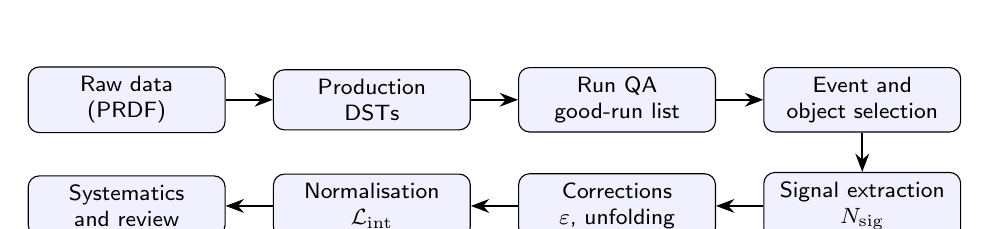
\begin{tikzpicture}[node distance=5mm and 6mm, every node/.style={font=\footnotesize},
 box/.style={draw, rounded corners, fill=blue!6, minimum width=2.5cm, minimum height=7mm, align=center},
 arr/.style={-{Stealth}, thick}]
\node[box] (raw) {Raw data\\(PRDF)};
\node[box, right=of raw] (dst) {Production\\DSTs};
\node[box, right=of dst] (qa) {Run QA\\good-run list};
\node[box, right=of qa] (ev) {Event and\\object selection};
\node[box, below=of ev] (sig) {Signal extraction\\$N_{\rm sig}$};
\node[box, left=of sig] (corr) {Corrections\\$\varepsilon$, unfolding};
\node[box, left=of corr] (norm) {Normalisation\\$\mathcal{L}_{\rm int}$};
\node[box, left=of norm] (sys) {Systematics\\and review};
\draw[arr] (raw)--(dst); \draw[arr] (dst)--(qa); \draw[arr] (qa)--(ev); \draw[arr] (ev)--(sig);
\draw[arr] (sig)--(corr); \draw[arr] (corr)--(norm); \draw[arr] (norm)--(sys);
\end{tikzpicture}\\[2pt]
{\small Figure 1 (schematic): the analysis chain. Each box is one section of this module.}
\end{center}

\connectbox{Your Run-24 $p$+$p$ $\pi^0$/$\eta$ analysis (module \texttt{pi0EtaAnalysisPP24} on \texttt{DST\_CALOFITTING}) is an
instance of Eq.~(\ref{eq:master}). $N_{\rm sig}$ comes from your diphoton mass fits; $\mathcal{L}_{\rm int}$ from GL1 scalers of the MB
bit (bit 10) divided by the MBD cross section; $\varepsilon$ from PYTHIA8 with EMCal smearing; and the Photon-3/4 triggers (bits 29/30)
need a turn-on correction and a prescale-aware luminosity. Keep this table open while you read; at the end you will turn it into your
error budget.}

%======================================================================
\section{Run QA and good-run lists}
\hd{Goal} Decide, run by run, whether the data are fit for your analysis, and record the decision so that it is reproducible.

\hd{Physics / concepts} A \emph{run} is a continuous period of data taking with fixed detector configuration, typically up to an hour.
Within a run the trigger set, prescales, high-voltage and readout are nominally constant. This makes the run the natural unit for
quality decisions. Problems that make a run unusable include: a subsystem off or partly off; wrong calibration or timing; hot or dead
regions; a beam condition (for example large background) that changes the event mix; a DAQ or GL1 problem that corrupts scalers.

The logic of run QA is statistical. Under stable conditions, a normalised distribution (hits per event versus $\phi$, mean cluster energy,
$\pi^0$ peak position) should be the same in every run up to statistical fluctuations. A run is suspicious if it deviates from the
reference by more than its statistical error allows.

\hd{A worked QA recipe from the school} [S33] did run QA for a silicon-plus-calorimeter $J/\psi$ analysis with these steps:
\begin{enumerate}
\item Normalise every QA histogram by the number of events (or tracks) in the run, so runs of different length can be compared.
\item Build a reference by averaging the normalised histograms of runs that look good: $\bar h_i = \frac{1}{R}\sum_{r=1}^{R} h_{r,i}$
for bin $i$ and $R$ runs.
\item For each run form the bin-by-bin ratio $\rho_{r,i} = h_{r,i}/\bar h_i$. A good run gives $\rho \approx 1$ in every bin.
\item Fit $\rho_{r,i}$ with a straight line (or a constant) and use $\chi^2/\mathrm{ndf}$ as the figure of merit. Good runs cluster
near $\chi^2/\mathrm{ndf}\approx 1$; bad runs (for example, an INTT ladder missing from the $\phi$ hit map) stand far out.
\item Check matching variables too: the track-to-EMCal residuals $d\phi$ and $dz$ should peak at zero in every run; a shifted peak
signals a misalignment or a bad calibration in that run.
\end{enumerate}

Why the ratio-and-fit method works: if $h_{r,i}$ has Poisson error $\sqrt{n_{r,i}}$ and the reference is built from many runs, the
reference error is negligible. Then $(\rho_{r,i}-1)/\sigma(\rho_{r,i})$ is approximately a unit Gaussian for a good run, and the
$\chi^2$ of a constant fit follows a $\chi^2$ distribution with $(N_{\rm bins}-1)$ degrees of freedom. A dead region adds a large,
localised deficit and $\chi^2/\mathrm{ndf}$ jumps.

\conceptbox{Worked example (toy)}{A hit map has 64 $\phi$ bins with about 2500 hits per bin per run. One run has one ladder dead,
covering 4 bins with zero hits. Each dead bin contributes $(0-1)^2/(1/\sqrt{2500})^2 = 2500$ to $\chi^2$. Four bins give
$\chi^2 \approx 10^4$ for 63 degrees of freedom, so $\chi^2/\mathrm{ndf}\approx 160$. A healthy run gives $\chi^2/\mathrm{ndf}\approx 1\pm0.18$
(the width is $\sqrt{2/63}$). The separation is enormous; the method cannot miss a dead ladder. It can miss a 2\% gain drift spread
over all bins, because a 2\% constant shift is absorbed by the fitted constant. That is why you also monitor absolute quantities such as
the mean or the $\pi^0$ peak position.}

\hd{How it is done in sPHENIX} Run QA happens at three levels.
\begin{itemize}
\item \emph{Online and shift level.} Shift crews and online monitoring flag runs during data taking (Module 5). The run database
records run type, duration, trigger configuration and detector status.
\item \emph{Production QA.} Each production pass fills standard QA histograms per run. For the calorimeters these come from QA
modules in \texttt{coresoftware} (for example \texttt{CaloValid}; check the current source for the exact list). Subsystem experts
publish run-quality flags and lists.
\item \emph{Analysis-level QA.} Each analysis adds its own checks: for a $\pi^0$ analysis, the run-by-run $\pi^0$ peak position and
width, the number of clusters per event, the fraction of masked towers, and the per-run trigger rates.
\end{itemize}
A \emph{good-run list} is then the intersection of the collaboration-level lists for the subsystems you use, your analysis-level cuts,
and practical requirements (for example a minimum number of events, the presence of the triggers you need with valid scalers, and a
magnetic-field state). The list must be a versioned text file kept with your code, with a reason recorded for each rejected run.

\begin{center}
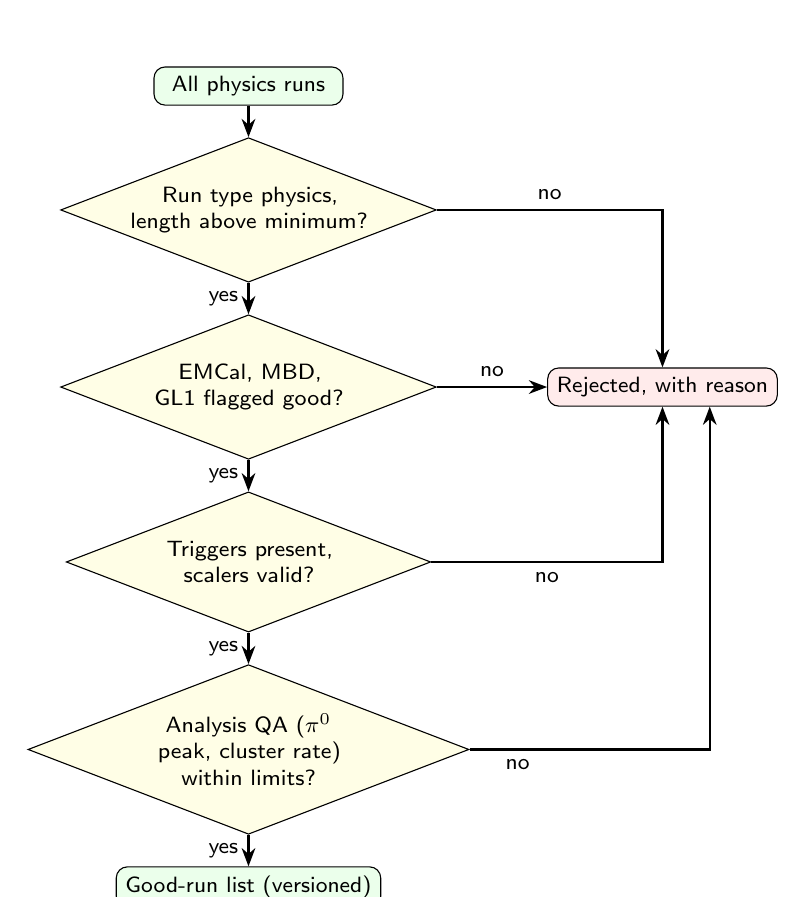
\begin{tikzpicture}[node distance=4mm, every node/.style={font=\footnotesize},
 q/.style={draw, diamond, aspect=2.6, fill=yellow!10, inner sep=1pt, align=center, text width=3.0cm},
 ok/.style={draw, rounded corners, fill=green!8, align=center, minimum width=2.4cm},
 no/.style={draw, rounded corners, fill=red!8, align=center, minimum width=2.4cm},
 arr/.style={-{Stealth}, thick}]
\node[ok] (all) {All physics runs};
\node[q, below=of all] (q1) {Run type physics, length above minimum?};
\node[q, below=of q1] (q2) {EMCal, MBD, GL1 flagged good?};
\node[q, below=of q2] (q3) {Triggers present, scalers valid?};
\node[q, below=of q3] (q4) {Analysis QA ($\pi^0$ peak, cluster rate) within limits?};
\node[ok, below=of q4] (good) {Good-run list (versioned)};
\node[no, right=1.4cm of q2] (rej) {Rejected, with reason};
\draw[arr] (all)--(q1); \draw[arr] (q1)--node[left]{yes}(q2); \draw[arr] (q2)--node[left]{yes}(q3);
\draw[arr] (q3)--node[left]{yes}(q4); \draw[arr] (q4)--node[left]{yes}(good);
\draw[arr] (q1.east)-|node[pos=0.25,above]{no}(rej.north);
\draw[arr] (q2.east)--node[above]{no}(rej.west);
\draw[arr] (q3.east)-|node[pos=0.25,below]{no}(rej.south);
\draw[arr] (q4.east)-|node[pos=0.1,below]{no}([xshift=6mm]rej.south);
\end{tikzpicture}\\[2pt]
{\small Figure 2 (schematic): a run-selection flow chart. Your checkpoint exercise asks you to write the real version for your analysis.}
\end{center}

\hd{Checks} Plot every QA figure of merit versus run number; look for steps (a calibration change or hardware intervention) and drifts
(gain change, ageing). Check that the list of rejected runs is stable when you change the reference sample. Check that the total
luminosity you keep is what you expect from the run log.

\pitfallbox{\begin{itemize}
\item Building the reference from all runs including bad ones; the reference is then biased. Iterate: build, reject outliers, rebuild.
\item Using QA cuts that depend on the signal you measure (for example rejecting runs with ``too few'' $\pi^0$ per event). This biases
the cross section. Cut on detector quantities, not on the physics result.
\item Forgetting that tower masks change with run. A run can be ``good'' but have a larger dead area; the acceptance must then be
computed with the right mask per run, or weighted by luminosity.
\item Keeping a good-run list only on your laptop. Reviewers will ask for it; version it with the code.
\end{itemize}}

\connectbox{For Run-24 $p$+$p$, record per run: the MB and Photon-3/4 scaled and live counts, the number of events passing your vertex
cut, the fitted $\pi^0$ mass and width in two fixed $p_T$ bins, and the number of masked EMCal towers. The $\pi^0$ peak position is a
direct monitor of the EMCal energy scale; a run whose peak is off by more than your scale uncertainty either needs a run-dependent
correction or rejection. This is exactly the per-run monitoring that your Tower Slope calibration work feeds.}

%======================================================================
\section{Triggers: selection, prescales and efficiency}
\hd{Goal} Know which events your trigger selected, how many it threw away, and with what efficiency it accepted signal.

\hd{Physics / concepts} RHIC has 120 bunch buckets per ring, so bunches cross every $\approx106$~ns, a crossing rate of about
9.4~MHz [S13]. sPHENIX cannot record every crossing; the trigger decides. The Global Level-1 (GL1) system receives trigger inputs
(MBD coincidences, ZDC, photon and jet triggers from the calorimeter trigger system, random and clock triggers) and forms up to
several dozen trigger bits. For every bit GL1 keeps three counters [S13]:
\begin{itemize}
\item \textbf{raw}: how many crossings fired the bit;
\item \textbf{live}: how many of those arrived while the DAQ could accept an event (not busy);
\item \textbf{scaled}: how many were actually recorded after prescaling.
\end{itemize}
A \emph{scaledown} (prescale) $s$ means that only one in $(s+1)$ live triggers is recorded, so
$N_{\rm live} \approx (s+1)\,N_{\rm scaled}$; [S13] wrote this as scaledown $=$ live/scaled $- 1$. The live fraction
$N_{\rm live}/N_{\rm raw}$ measures dead time.

\hd{Equivalent sampled MB events} A rare-signal trigger (Photon-3) is usually unprescaled or lightly prescaled; the MB trigger is
heavily prescaled. To normalise photon-triggered data you need the number of MB events the photon trigger \emph{sampled}. Think of it this way. In a run where both bits were live for the
same crossings, the photon-triggered sample is equivalent to
$N_{\rm MB}^{\rm live}/(s_\gamma+1)$ MB events, because the photon trigger examined every live MB crossing (it is a subset condition
when the photon trigger requires the MB condition) and kept one in $(s_\gamma+1)$. Hence
\begin{equation}
N_{\rm MB}^{\rm equiv}(\gamma\ \mathrm{sample}) = \sum_{\rm runs}\frac{N^{\rm live}_{\rm MB}}{s_\gamma + 1}.
\label{eq:equiv}
\end{equation}
Use live (not raw) counts in the numerator because dead crossings were seen by neither trigger. Whether the photon trigger in a given
run included the MB condition is a configuration fact you must check in the trigger setup for that period.

\conceptbox{Worked example (toy)}{In one run, the MB bit has $N^{\rm live}_{\rm MB}=4.0\times10^{8}$ and scaledown 399, so
$N^{\rm scaled}_{\rm MB}= 10^6$ events are on tape. Photon-3 has scaledown 0 and records $2\times10^{6}$ events. The MB sample
represents $10^6$ events; the Photon-3 sample represents $4.0\times10^8$ sampled MB events (Eq.~\ref{eq:equiv} with $s_\gamma=0$). A
$\pi^0$ spectrum from Photon-3 is normalised by $4.0\times10^8$, not by $2\times10^6$. If a later run has Photon-3 scaledown 1, its
equivalent count is halved. You sum runs one by one; never multiply a total by an average prescale.}

\hd{Trigger efficiency and turn-on} A calorimeter photon trigger fires when an energy sum in a trigger tile exceeds a threshold
(nominally a few GeV, hence ``Photon-3/4''). The trigger sees uncalibrated, coarsely summed energy, so its efficiency versus offline
cluster energy is not a step but a smooth \emph{turn-on} curve. Measure it with an unbiased reference sample:
\begin{equation}
\varepsilon_{\rm trig}(E) = \frac{N(\mbox{MB-triggered events with leading cluster } E \mbox{ that also fired } \gamma)}
{N(\mbox{MB-triggered events with leading cluster } E)} ,
\end{equation}
using the GL1 \emph{live} (pre-scale) trigger vector so that the photon decision is known even when the photon bit was not the reason
the event was kept. Fit with an error function,
$\varepsilon(E) = \frac{\varepsilon_0}{2}\left[1+\mathrm{erf}\!\left(\frac{E-E_{50}}{\sqrt{2}\,w}\right)\right]$, where $E_{50}$ is the
50\% point, $w$ the width, and $\varepsilon_0$ the plateau. Analyses normally use only the plateau region, where the correction is close
to one and its uncertainty small. Binomial errors near $\varepsilon\approx1$ are badly behaved; use Clopper--Pearson or Bayesian
intervals (ROOT \texttt{TEfficiency}).

For a $\pi^0$ the relevant quantity is the trigger efficiency versus \emph{$\pi^0$} $p_T$, not versus cluster energy. The trigger
fires on the more energetic photon (or the merged cluster); the leading-photon energy fraction varies with the decay asymmetry
$\alpha=|E_1-E_2|/(E_1+E_2)$, which is uniform on $[0,1]$ for $\pi^0\to\gamma\gamma$. So the $\pi^0$ turn-on is wider than the cluster
turn-on, and is best computed by folding the measured cluster turn-on with simulated decays, or measured directly in data as the
fraction of MB-triggered $\pi^0$ candidates that also fired the photon bit.

\hd{Vertex and MB efficiency} Your normalisation counts MB events within a vertex window, and your signal counts $\pi^0$ in the same
window. Two efficiencies enter. First, $\varepsilon_{\rm MBD}^{\rm sig}$: the probability that an event containing your signal fires
the MBD coincidence. Hard-scattering events have more forward particles, so this is higher than for the average inelastic event.
Second, the vertex-reconstruction and $|z|$-cut efficiency. [S17] showed that, for prompt photons, this combined factor is far from one
and is a major correction; it is estimated with PYTHIA passed through the full simulation, and its uncertainty enters the systematics.

\hd{How it is done in sPHENIX} The GL1 information is stored per event in the \texttt{Gl1Packet} object (raw, live and scaled trigger
vectors and per-bit scaler counters). Helper classes such as \texttt{TriggerAnalyzer} decode trigger names and prescales from the
database (check the current \texttt{coresoftware} for exact class and method names). Per-run scaler totals are also stored in the run
database, which is what luminosity bookkeeping should use.

\pitfallbox{\begin{itemize}
\item Normalising by the number of recorded events instead of the sampled MB count.
\item Using the scaled vector to measure trigger efficiency: the scaled bit is zero for most events in which the trigger fired.
\item Measuring the turn-on in a sample that is itself biased toward high-energy clusters (for example, a jet-triggered sample).
\item Forgetting that the photon trigger in some periods included an MBD requirement and in others did not; the denominator changes.
\item Treating the plateau as exactly 100\%. Measure it and assign the statistical error of the plateau fit as a systematic.
\end{itemize}}

\connectbox{Write a short function that, per run, reads $N^{\rm live}$ and $s$ for bits 10, 29 and 30 and returns the equivalent MB
counts per trigger. Combine Photon-3 and Photon-4 only through a rule that avoids double counting (for example: use each trigger only in
the $\pi^0$ $p_T$ range where it is on plateau, and normalise each range by its own equivalent count). Measure the $\pi^0$ turn-on
directly from MB events using the live trigger vector, and compare with the folding method. The difference is a systematic.}

%======================================================================
\section{Luminosity and the Vernier scan}
\hd{Goal} Turn a count of MB events into an integrated luminosity with a known uncertainty, and understand where the MBD cross section
comes from.

\subsection{Luminosity from beam parameters}
\hd{Physics / concepts} The instantaneous luminosity $\mathcal{L}$ is defined by $R = \sigma\,\mathcal{L}$: the rate of any process
equals its cross section times $\mathcal{L}$. For two bunched beams with $N_b$ colliding bunch pairs, revolution frequency $f_{\rm rev}$,
and bunch populations $N_1$, $N_2$,
\begin{equation}
\mathcal{L} = N_b\,f_{\rm rev}\,N_1 N_2 \int \rho_1(x,y)\,\rho_2(x,y)\,dx\,dy ,
\end{equation}
where $\rho_{1,2}$ are the normalised transverse density profiles. Assume Gaussian profiles with widths $\sigma_{x1},\sigma_{y1}$ and
$\sigma_{x2},\sigma_{y2}$, and displace beam 2 by $(\delta_x,\delta_y)$. The overlap integral factorises into $x$ and $y$. In $x$,
\begin{equation}
\int \frac{e^{-x^2/2\sigma_{x1}^2}}{\sqrt{2\pi}\sigma_{x1}}\,\frac{e^{-(x-\delta_x)^2/2\sigma_{x2}^2}}{\sqrt{2\pi}\sigma_{x2}}\,dx
= \frac{1}{\sqrt{2\pi}\,\Sigma_x}\exp\!\left(-\frac{\delta_x^2}{2\Sigma_x^2}\right),\qquad \Sigma_x^2=\sigma_{x1}^2+\sigma_{x2}^2 .
\end{equation}
(The product of two Gaussians integrates to a Gaussian in the separation whose variance is the sum of the variances; this is the
convolution theorem for Gaussians.) Therefore
\begin{equation}
\mathcal{L}(\delta_x,\delta_y) = \frac{N_b f_{\rm rev} N_1 N_2}{2\pi\,\Sigma_x\Sigma_y}\,
\exp\!\left(-\frac{\delta_x^2}{2\Sigma_x^2}-\frac{\delta_y^2}{2\Sigma_y^2}\right).
\label{eq:vernier}
\end{equation}
At head-on collision ($\delta=0$) this is the formula quoted in [S41]:
$\mathcal{L}_0 = N_b f_{\rm rev} N_1N_2/(2\pi\Sigma_x\Sigma_y)$ with $\Sigma_{x}=\sqrt{\sigma_{x1}^2+\sigma_{x2}^2}$.

\subsection{The Vernier scan}
The products $N_1N_2$ are measured by beam-current monitors operated by the accelerator. The unknowns are the overlap widths
$\Sigma_x,\Sigma_y$. A \emph{Vernier scan} measures them directly [S41]: the beams are stepped across each other, first horizontally,
then vertically, and at each offset the rate of a detector coincidence (MBD or ZDC) is recorded. By Eq.~(\ref{eq:vernier}) the rate
versus offset is a Gaussian whose width is exactly $\Sigma_x$ (or $\Sigma_y$). With $\Sigma_x$, $\Sigma_y$ and $N_1N_2$ one has
$\mathcal{L}_0$, and the detector cross section follows from the head-on rate:
\begin{equation}
\sigma_{\rm MBD} = \frac{R_{\rm MBD}(\delta=0)}{\mathcal{L}_0}.
\end{equation}
The key insight is that $\sigma_{\rm MBD}$ is a property of the detector and trigger (acceptance times efficiency times the
inelastic cross section), and stays fixed as long as the detector does. Once it is known, every later MB count converts to luminosity:
$\mathcal{L}_{\rm int} = N_{\rm MB}/\sigma_{\rm MBD}$.

\conceptbox{Worked example (toy numbers, not sPHENIX values)}{Take $N_b=111$, $f_{\rm rev}=78$~kHz (the RHIC revolution frequency is
about 78~kHz), $N_1=N_2=1.5\times10^{11}$, and $\sigma_{x}=\sigma_{y}=0.15$~mm for each beam, so $\Sigma=0.212$~mm $=0.0212$~cm.
Then $\mathcal{L}_0 = 111\times7.8\times10^{4}\times2.25\times10^{22}/(2\pi\times4.5\times10^{-4}\,\mathrm{cm^2})
\approx 6.9\times10^{31}\,\mathrm{cm^{-2}s^{-1}}$. A toy detector cross section of 20~mb ($2\times10^{-26}$~cm$^2$) gives a rate of
1.4~MHz. Dividing by the crossing rate $N_b f_{\rm rev}\approx8.7$~MHz gives a mean of $\mu\approx0.16$ MBD-visible collisions per
crossing; pile-up is not negligible at this luminosity.}

\subsection{Corrections}
[S41] listed the corrections that turn the raw scan into a cross section. Each has a clear physical origin.
\begin{enumerate}
\item \textbf{Beam intensity.} $N_1N_2$ decays during the scan. Normalise the rate at each step by the product of the bunch
intensities at that time.
\item \textbf{Multiple collisions and accidentals.} The MBD counts \emph{crossings} with a north--south coincidence, not collisions.
Let $\mu$ be the mean number of collisions per crossing (Poisson). Let a single collision fire both sides with probability
$\varepsilon_{NS}$, only north with $\varepsilon_N$, only south with $\varepsilon_S$. The probability that the north side fires in a
crossing is $1-e^{-\mu(\varepsilon_{NS}+\varepsilon_N)}$, similarly for south. By inclusion--exclusion, the coincidence probability is
\begin{equation}
P_{NS}(\mu) = 1 - e^{-\mu(\varepsilon_{NS}+\varepsilon_N)} - e^{-\mu(\varepsilon_{NS}+\varepsilon_S)} + e^{-\mu(\varepsilon_{NS}+\varepsilon_N+\varepsilon_S)} .
\end{equation}
For small $\mu$ this is $\mu\varepsilon_{NS}$ (true coincidences); the quadratic term contains the accidental coincidences in which
the north hit comes from one collision and the south hit from another. One measures $P_{NS}$ per bunch and solves for $\mu$. In the
simplest case ($\varepsilon_N=\varepsilon_S=0$) the inversion is $\mu\varepsilon_{NS} = -\ln(1-P_{NS})$.
\item \textbf{Bunch-by-bunch treatment.} Bunches differ in intensity and size; the analysis is done per bunch pair, using
GL1 per-bunch counters, and non-colliding bunches give the background level.
\item \textbf{Hourglass effect.} Near the interaction point the beam size varies along $z$: $\sigma(z)=\sigma^*\sqrt{1+(z/\beta^*)^2}$,
with $\beta^*$ the beta function at the focus. Long bunches therefore collide partly where the beams are wider, and the effective
luminosity is lower than Eq.~(\ref{eq:vernier}) with $\sigma^*$. The correction is computed with a model of the bunch length and
$\beta^*$; it also affects the shape of the vertex distribution [S41].
\item \textbf{Non-Gaussian tails.} The ZDC, which detects spectator neutrons at very forward angles, is more sensitive to beam halo
and tails; [S41] used a double Gaussian for the ZDC scan shape. The overlap integral must then be computed numerically.
\item \textbf{Vertex acceptance.} The cross section can be defined for all vertices or for a vertex window. Analyses that cut
$|z|<z_{\rm max}$ must use the cross section and MB count for the same window (or the fraction of MBD events inside the window).
\end{enumerate}
The MBD covers $3.51<|\eta|<4.61$ on both sides; it is the MB trigger and the luminosity monitor. The ZDC provides an independent
measurement. Agreement between them, and between scans in different years, is a strong check [S41].

\subsection{Integrated luminosity for an analysis}
For a trigger sample $T$,
\begin{equation}
\mathcal{L}_{\rm int}(T) = \frac{N^{\rm equiv}_{\rm MB}(T)}{\sigma_{\rm MBD}} ,
\end{equation}
with $N^{\rm equiv}_{\rm MB}$ from Eq.~(\ref{eq:equiv}), corrected for pile-up if one recorded MB crossing can contain more than one
collision. The relative uncertainty of $\sigma_{\rm MBD}$ is a \emph{global} (fully correlated) uncertainty on every point of your
spectrum. It is quoted separately from the point-to-point uncertainties. In a ratio such as $\eta/\pi^0$ from the same events it
cancels exactly.

\subsection{Relative luminosity in spin analyses}
For a transverse single-spin asymmetry $A_N = (\sigma_L-\sigma_R)/(\sigma_L+\sigma_R)$ (Module 1), what matters is not the absolute
luminosity but the ratio $\mathcal{R}=\mathcal{L}^{\uparrow}/\mathcal{L}^{\downarrow}$ of luminosities delivered in bunches of
opposite polarisation [S30]. With yields $N^{\uparrow}$, $N^{\downarrow}$ in one detector arm,
\begin{equation}
\epsilon_N = \frac{N^{\uparrow} - \mathcal{R}N^{\downarrow}}{N^{\uparrow} + \mathcal{R}N^{\downarrow}}, \qquad A_N=\frac{\epsilon_N}{P_{\rm beam}} .
\end{equation}
The \emph{square-root} formula combines left and right arms,
$\epsilon_N = (\sqrt{N_L^{\uparrow}N_R^{\downarrow}}-\sqrt{N_L^{\downarrow}N_R^{\uparrow}})/(\sqrt{N_L^{\uparrow}N_R^{\downarrow}}+\sqrt{N_L^{\downarrow}N_R^{\uparrow}})$;
both luminosity and acceptance cancel to first order. In practice one fits the azimuthal dependence $\epsilon(\phi)=\epsilon_N\sin\phi$
[S30]. The rapid bunch-by-bunch spin flip at RHIC is what makes these cancellations work: both spin states see the same detector within
microseconds.

\pitfallbox{\begin{itemize}
\item Using a cross section measured for one vertex window with MB counts for another.
\item Ignoring pile-up in high-luminosity runs. At $\mu=0.16$, about 8\% of crossings with a collision contain more than one.
\item Quoting the luminosity uncertainty inside the point-to-point error bars. It is a global scale.
\item Forgetting that scans are done at special times; changes to the MBD (thresholds, timing) after the scan change
$\sigma_{\rm MBD}$.
\end{itemize}}

\connectbox{Your normalisation is $\mathcal{L}_{\rm int}=N^{\rm equiv}_{\rm MB}/\sigma_{\rm MBD}$ with $N^{\rm equiv}_{\rm MB}$ from
GL1 live counts of bit 10 within your vertex window. Three things to document: (1) which $\sigma_{\rm MBD}$ value and vertex
definition you use, and its uncertainty (from the Run-24 Vernier analysis); (2) the per-run pile-up correction; (3) the efficiency of
the MBD trigger for events that contain a $\pi^0$ of given $p_T$, which is not the same as for average inelastic events. Point (3)
enters $\varepsilon$, not $\mathcal{L}$; do not count it twice.}

%======================================================================
\section{Centrality, Glauber modelling and event-plane corrections}
\hd{Goal} Classify A+A events by centrality, attach geometric quantities ($N_{\rm part}$, $N_{\rm coll}$, $T_{AA}$) to each class, and
understand detector corrections for event-plane observables.

\subsection{The Glauber model}
\hd{Physics / concepts} Nuclei are sampled as $A$ nucleons from a Woods--Saxon density
$\rho(r)\propto 1/(1+e^{(r-R)/a})$. For a random impact parameter $b$, two nucleons collide if their transverse distance $d$ satisfies
$\pi d^2<\sigma_{NN}^{\rm inel}$, with $\sigma_{NN}^{\rm inel}\approx42$~mb at $\sqrt{s_{NN}}=200$~GeV. Counting gives
$N_{\rm part}$ (nucleons that collided at least once) and $N_{\rm coll}$ (binary collisions). The nuclear overlap function is
$T_{AA}=N_{\rm coll}/\sigma_{NN}^{\rm inel}$. Soft particle production scales roughly with $N_{\rm part}$; hard processes scale
with $N_{\rm coll}$.

\subsection{Centrality from the MBD charge sum}
The MBD charge sum $Q$ is monotonic in multiplicity at forward rapidity, and therefore in $b$ on average. The standard procedure, used
in [S26] for O+O, is:
\begin{enumerate}
\item Generate $N_{\rm part}$ (or a number of ``ancestors'', e.g.\ $fN_{\rm part}+(1-f)N_{\rm coll}$) with a Monte Carlo Glauber.
\item Model the charge per ancestor as a negative binomial distribution (NBD),
\begin{equation}
P(n;\mu,k) = \frac{\Gamma(n+k)}{\Gamma(n+1)\Gamma(k)}\left(\frac{\mu}{k}\right)^{n}\left(1+\frac{\mu}{k}\right)^{-(n+k)} ,
\end{equation}
with mean $\mu$ and shape $k$. Convolve over ancestors to predict the $Q$ distribution.
\item Fit $\mu$, $k$ and the normalisation to the measured $Q$ distribution \emph{only in the region where the trigger is fully
efficient} (high $Q$).
\item Extrapolate to low $Q$. The ratio of measured to predicted events gives the MB trigger efficiency, i.e.\ the fraction of the
inelastic cross section the trigger sees.
\item Define centrality classes by integrating the fitted distribution from the top: the 0--10\% class is the 10\% of the total
inelastic cross section with the largest $Q$.
\item For each class, read $\langle N_{\rm part}\rangle$, $\langle N_{\rm coll}\rangle$ and $\langle T_{AA}\rangle$ from the Glauber
events falling in that class.
\end{enumerate}

\hd{How it is done in sPHENIX} \texttt{MbdReco} produces the calibrated MBD charges and times, and \texttt{GlobalVertexReco} the vertex.
\texttt{MinimumBiasClassifier} applies the offline MB definition and \texttt{CentralityReco} assigns the centrality from calibrated
cuts; both were named as the official modules in [S26]. They write MB and centrality information to the node tree (check the current
node names). Before official calibrations exist, analysts do the NBD--Glauber fit themselves, as [S26] did for the first O+O data.

\hd{Checks} The centrality distribution of MB events should be flat in the fully efficient range. The charge sum depends on the vertex
position (acceptance changes with $z$), so check the classes in several $z$ slices. Compare the generator's $N_{\rm part}$
distribution with a standalone Glauber calculation: [S26] found an unexpected structure at low $N_{\rm part}$ in one official
simulation sample, which would bias peripheral classes.

\conceptbox{From centrality to $R_{AA}$ and $R_{CP}$}{The nuclear modification factor compares a yield per event in a centrality class
with the $p$+$p$ cross section scaled by $T_{AA}$:
$R_{AA}(p_T) = \frac{1}{\langle T_{AA}\rangle}\,\frac{dN_{AA}/dp_T}{d\sigma_{pp}/dp_T}$.
Without a $p$+$p$ reference one uses the central-to-peripheral ratio
$R_{CP} = \frac{\langle N_{\rm coll}^{P}\rangle}{\langle N_{\rm coll}^{C}\rangle}\,\frac{Y_C}{Y_P}$.
In $R_{CP}$ the luminosity and many efficiencies cancel; the Glauber $N_{\rm coll}$ ratio and the peripheral MB efficiency do not.}

\subsection{Event-plane analysis as a model of detector corrections}
The azimuthal distribution relative to the $n$-th order symmetry plane is $dN/d\phi\propto1+2\sum_n v_n\cos[n(\phi-\Psi_n)]$. The
geometric reason is simple: in a non-central collision the overlap is almond shaped, pressure gradients are larger along the short
axis, and the fluid pushes more particles in that direction [S05, S34]. [S34] measured $v_2$ in Au+Au with the INTT and the MBD, and
the steps are a compact lesson in correcting detector effects.
\begin{enumerate}
\item \textbf{Flow vector.} $Q_x=\sum_i w_i\cos 2\phi_i/\sum_i w_i$, $Q_y=\sum_i w_i\sin 2\phi_i/\sum_i w_i$, and
$\Psi_2=\frac12\mathrm{atan2}(Q_y,Q_x)$; weights $w_i$ are charges or hit counts.
\item \textbf{Recentering.} Detector non-uniformity makes $\langle Q_x\rangle,\langle Q_y\rangle\neq0$ and $\Psi_2$ non-flat.
Replace $Q\to(Q-\langle Q\rangle)/\sigma_Q$ per centrality and vertex bin.
\item \textbf{Flattening.} Remove residual harmonics with a Fourier shift (Poskanzer--Voloshin method):
\[\Psi' = \Psi + \frac{1}{2}\sum_{k=1}^{N}\frac{2}{k}\left[-\langle\sin 2k\Psi\rangle\cos 2k\Psi + \langle\cos 2k\Psi\rangle\sin 2k\Psi\right].\]
A constant fit to the flattened distribution should give $\chi^2/\mathrm{ndf}\approx1$.
\item \textbf{Resolution.} A finite number of particles gives a smeared plane, so $v_2^{\rm obs}=v_2\,\langle\cos2(\Psi_2^{\rm meas}-\Psi_2)\rangle$.
With three detectors A, B, C (INTT, MBD south, MBD north),
\[R_A=\sqrt{\frac{\langle\cos2(\Psi_A-\Psi_B)\rangle\langle\cos2(\Psi_A-\Psi_C)\rangle}{\langle\cos2(\Psi_B-\Psi_C)\rangle}}.\] Then
$v_2=v_2^{\rm obs}/R$.
\item \textbf{Rapidity gap.} Particles and plane from different $\eta$ regions avoid autocorrelation and reduce non-flow (jets,
decays).
\item \textbf{Systematics.} Change the plane detector (MBD south only, north only, INTT halves) and take the spread [S34].
\end{enumerate}

\pitfallbox{\begin{itemize}
\item Fitting the NBD over the inefficient low-$Q$ region; the efficiency then comes out wrong and all peripheral classes shift.
\item Using centrality classes from one vertex range with events from another.
\item Treating the Glauber $N_{\rm coll}$ as exact: its uncertainty (from $\sigma_{NN}$, nuclear shape, MB efficiency) enters $R_{AA}$
and $R_{CP}$ as a correlated systematic.
\item Forgetting pile-up: two peripheral collisions in one crossing look like a mid-central one.
\end{itemize}}

\connectbox{In your Au+Au $\pi^0$ $R_{CP}$, the peripheral class carries the largest geometric uncertainty because the MB efficiency is
not 100\% and the NBD extrapolation matters most there. The event-plane machinery also gives the $\pi^0$ $v_2$, which the Bulk TG
extracted already from commissioning data [S05]. Your event-mixing background would then need mixing in bins of event-plane angle as
well as centrality and vertex.}

%======================================================================
\section{Efficiency, acceptance and embedding}
\hd{Goal} Compute the probability that a produced signal particle ends up counted, as a function of the kinematic variables of your
measurement, and verify that the simulation used for it describes the data.

\hd{Physics / concepts} Factorise the total efficiency into pieces that can be checked separately,
\begin{equation}
\varepsilon = A\times\varepsilon_{\rm reco}\times\varepsilon_{\rm ID}\times\varepsilon_{\rm trig}\times\varepsilon_{\rm vtx} ,
\end{equation}
where $A$ is geometric acceptance (both photons inside the live EMCal), $\varepsilon_{\rm reco}$ the clustering and pairing
efficiency, $\varepsilon_{\rm ID}$ the efficiency of shower-shape or isolation cuts, and the last two the trigger and vertex pieces of
Section 3. [S17] showed this decomposition for prompt photons: reconstruction, identification and isolation efficiencies multiply.
The signal must be defined at truth level first: which particles count (for example primary $\pi^0$ excluding those from weak decays
of $K^0_S$), in which kinematic range. [S26] stressed this with the definition of a primary charged particle.

\subsection{Three kinds of simulation}
\begin{itemize}
\item \textbf{Single-particle gun.} One particle per event at a chosen $p_T$, $\eta$, vertex. Clean, fast, and gives response
functions directly. It lacks the underlying event, so isolation and occupancy effects are missing. It must be reweighted to a
realistic spectrum when used for bin-integrated efficiencies.
\item \textbf{Full event generator (PYTHIA8, HIJING).} Realistic event environment and correlated particles. For $p$+$p$ this is
the standard choice. Generator-level problems (wrong $N_{\rm part}$, wrong multiplicity) propagate into corrections, so check the
generator against data.
\item \textbf{Embedding.} Simulated signal particles are inserted into \emph{real} data events, then reconstructed together. The
background, noise and occupancy are real by construction. In Fun4All, embedding uses a second node tree for the simulated hits that
are merged with the data before reconstruction [S14]. Embedding is essential in Au+Au, where occupancy changes efficiencies and
resolutions with centrality.
\end{itemize}

\subsection{The correction-factor method}
For counting analyses one often uses one combined factor. [S26] corrected INTT tracklet counts with
\begin{equation}
f(\eta,\mathrm{cent}) = \frac{N_{\rm reco}^{\rm MC}(\eta,\mathrm{cent})}{N_{\rm truth}^{\rm MC}(\eta,\mathrm{cent})},\qquad
\frac{dN_{\rm ch}}{d\eta}=\frac{N^{\rm data}_{\rm reco}}{f\,\Delta\eta\,N_{\rm ev}} .
\end{equation}
This ratio absorbs acceptance, efficiency, secondaries and residual background at once. Its validity rests on the simulation
reproducing the data inputs: [S26] reweighted the MC vertex distribution by the data/MC ratio, and [S25] applied the dead-channel map
measured in data to the simulation at digitisation. These two steps illustrate the general rule: \emph{make the simulation look like
the data in every variable the efficiency depends on}.

\subsection{Why steep spectra make resolution matter}
\conceptbox{Derivation and worked example}{Let the true spectrum be $dN/dp_T=Ap_T^{-m}$. Suppose the measured momentum is
$p'=(1+s)p$ (a scale offset $s$). Then the measured spectrum at fixed $p'$ is $A(1+s)^{m-1}p'^{-m}$: the yield in a bin rises by
$(1+s)^{m-1}$. Now add a Gaussian relative resolution $r$, $p'=p(1+xr)$ with $x\sim N(0,1)$. Averaging over $x$,
$g(p')=Ap'^{-m}\,\mathrm{E}[(1+xr)^{m-1}]\approx Ap'^{-m}\left[1+\tfrac{(m-1)(m-2)}{2}r^2\right]$.
For a $\pi^0$ invariant spectrum falling like $p_T^{-8}$, $dN/dp_T\propto p_T^{-7}$, so $m=7$:
a 1\% scale offset changes the yield by $1.01^{6}-1\approx6\%$, and a 10\% resolution raises the yield by about
$15\times0.01=15\%$. Small calorimeter mis-calibrations are therefore large cross-section effects, and the MC resolution must match the
data. This is why [S43] stressed that RHIC jet spectra, which are much steeper than at the LHC, need very careful treatment.}

\subsection{The $\pi^0$ and $\eta$ in the EMCal}
For a two-body decay of a particle of mass $m$ and energy $E$, the minimum opening angle is $\theta_{\min}\approx2m/E$ (exact:
$\sin(\theta_{\min}/2)=m/E$). The EMCal has $256$ towers in $\phi$, so one tower spans $2\pi/256\approx0.0245$~rad, and about the
same in $\eta$ (96 towers over $|\eta|<1.1$). For a 10~GeV $\pi^0$, $\theta_{\min}\approx0.027$~rad, about one tower: the two showers
start to overlap and the clusterizer must split them. For an $\eta$ at 10~GeV, $\theta_{\min}\approx0.11$~rad, about 4.5 towers, so
merging is not yet an issue. The template-based splitting in \texttt{RawClusterBuilderTemplate} redistributes energy between local
maxima using a shower profile [S17]; its behaviour controls your high-$p_T$ $\pi^0$ efficiency and must be modelled in simulation.

\hd{How it is done in sPHENIX} Simulations are run with \texttt{PHG4Reco} (Geant4) in Fun4All macros such as
\texttt{Fun4All\_G4\_sPHENIX.C}, then digitised and reconstructed with the same calorimeter chain as data (towers in
\texttt{TowerInfo} containers, clusters from \texttt{RawClusterBuilderTemplate}). Official production samples exist for PYTHIA8 and
HIJING; embedding productions exist for some signals (check the production pages for current samples).

\hd{Checks} Compare data and MC for every variable entering a cut (cluster energy, shower width, $\chi^2$, timing). Compare the
$\pi^0$ peak position and width versus $p_T$ in data and MC; a mismatch means extra smearing or a scale shift is needed. Do a
\emph{closure test}: apply your full correction chain to an MC sample treated as data and recover the truth.

\pitfallbox{\begin{itemize}
\item Computing efficiency with a flat-$p_T$ gun and applying it to a steep spectrum, without reweighting.
\item Different truth definitions in numerator and denominator (for example, including feed-down in one and not the other).
\item Applying the data tower masks in reconstruction but not in the simulation, or vice versa.
\item Using one MC energy scale for all runs when the data scale drifted with run.
\end{itemize}}

\connectbox{Your PYTHIA8 efficiency with EMCal smearing is the $\varepsilon_{\rm reco}\times\varepsilon_{\rm ID}$ part. Two checks
follow directly from this section. First, the extra smearing must be tuned so that the MC $\pi^0$ width matches data in each $p_T$ bin;
the residual mismatch becomes the energy-resolution systematic. Second, the scale must match the data $\pi^0$ peak; with $m\approx7$ a
residual 1\% offset is a 6\% yield systematic. Your Tower Slope MC studies are, in this language, a test of how well tower-level gain
non-uniformities are removed before these global checks.}

%======================================================================
\section{Unfolding basics}
\hd{Goal} Correct a measured spectrum for bin-to-bin migration caused by finite resolution, without amplifying statistical noise.

\hd{Physics / concepts} Write the measured counts in reconstructed bin $i$ as
\begin{equation}
m_i = \sum_j R_{ij}\,t_j + b_i ,\qquad R_{ij}=P(\mbox{reco in } i\mid \mbox{true in } j),\qquad \sum_i R_{ij}=\varepsilon_j ,
\end{equation}
where $t_j$ is the true spectrum, $b_i$ the fakes (reconstructed objects with no true counterpart in the fiducial range), and
$\varepsilon_j$ the efficiency (the ``misses'' are $1-\varepsilon_j$). The response matrix $R$ comes from simulation by matching
reconstructed and true objects.

\conceptbox{Why not just invert $R$? (toy)}{Take two bins and $R=\begin{pmatrix}0.8&0.2\\0.2&0.8\end{pmatrix}$. Then
$R^{-1}=\frac{1}{0.6}\begin{pmatrix}0.8&-0.2\\-0.2&0.8\end{pmatrix}$. For $m=(100,100)$ we get $t=(100,100)$. A statistical
fluctuation to $m=(110,90)$ gives $t=(116.7,83.3)$: a 10-count fluctuation became 16.7. With stronger migration,
$R=\begin{pmatrix}0.6&0.4\\0.4&0.6\end{pmatrix}$, the determinant is 0.2 and the same fluctuation becomes 50 counts. Inversion is
unbiased but its variance explodes as migration grows. Unfolding methods trade a small bias for a large reduction in variance; this
trade is called \emph{regularisation}.}

\subsection{Bin-by-bin correction}
If bins are much wider than the resolution, most events stay in their bin. Then a simple factor
$C_i = t_i^{\rm MC}/m_i^{\rm MC}$ applied as $t_i = C_i\,m_i$ works. It is exact only if the MC spectrum shape is correct, because $C_i$
depends on how many events migrate in from neighbours. The test is the bin \emph{purity} (fraction of reconstructed events in bin $i$
whose true value is also in bin $i$) and \emph{stability}; if both are high (say above 80\%), bin-by-bin is acceptable and its shape
dependence is checked by reweighting the MC.

\subsection{Iterative Bayesian (D'Agostini) unfolding}
This method, used in the sPHENIX jet and photon analyses [S43, S17] through the RooUnfold package, applies Bayes' theorem. Start with a
prior $p_j$ (normally the MC truth). The probability that an event seen in bin $i$ came from true bin $j$ is
\begin{equation}
P(j\mid i) = \frac{R_{ij}\,p_j}{\sum_k R_{ik}\,p_k} .
\end{equation}
Then distribute the background-subtracted data and correct for efficiency:
\begin{equation}
\hat t_j = \frac{1}{\varepsilon_j}\sum_i P(j\mid i)\,(m_i-b_i) .
\end{equation}
Use $\hat t$ as the new prior and repeat. Few iterations stay close to the prior (strong regularisation, more bias); many iterations
approach matrix inversion (less bias, more noise). The number of iterations is chosen by convergence (the change between iterations
falls below the statistical error) and by closure tests. Statistical errors come from bootstrapping or toy variations of the data
and of the response matrix.

\subsection{Validation}
\begin{itemize}
\item \textbf{Full closure.} Unfold the MC reconstructed spectrum with the response from the same MC; you must recover the truth.
This tests the code, not the method.
\item \textbf{Half closure.} Split the MC into independent halves; build $R$ from one and unfold the other. This tests statistical
robustness [S17].
\item \textbf{Prior or shape closure.} Reweight the MC truth so that its reconstructed spectrum matches data, rebuild $R$ and
unfold again. The change is the prior-dependence systematic [S17, S43].
\item \textbf{Refolding.} Fold the unfolded result with $R$ and compare with the measured data; the $\chi^2$ must be acceptable.
\item \textbf{Iteration variation.} Change the number of iterations by one or two; the change is a systematic [S43, S17].
\end{itemize}
[S43] posed the key question: how do we know unfolding can be applied to data? The answer is that $R$ must be validated against data.
For jets this was done with data-driven resolution and scale measurements: the dijet momentum imbalance and bisector methods measure the
jet energy resolution in data, after extrapolating to events with no hard third jet, because soft radiation adds isotropically while
detector smearing acts only on the jet magnitude. The data--MC difference was then applied as extra smearing in the MC. Photon--jet and
multijet balance constrain the jet energy scale [S43].

\hd{The high-side response problem} [S43] showed a subtle failure. If a small fraction of low-$p_T$ truth objects is reconstructed at
much higher $p_T$ (for example because a wrong vertex position, such as a forced $z=0$, shifts the measured transverse energy), a steep
spectrum turns this tiny tail into a large fraction of the high-$p_T$ reconstructed yield. The unfolded result then depends on how well
the simulation models a rare detector effect. The robust fix is to remove the cause (better vertexing) rather than to trust the matrix.

\pitfallbox{\begin{itemize}
\item Choosing the iteration count by eye on data alone.
\item Truth binning that does not extend below the reconstructed range: low-$p_T$ truth that migrates up is then treated as fakes or
lost. [S17] used truth bins starting well below the lowest reconstructed bin for this reason.
\item Unfolding a spectrum that still contains background; subtract or purity-correct first.
\item Forgetting that unfolded bins are correlated; use the covariance matrix in fits and comparisons.
\end{itemize}}

\connectbox{For $\pi^0$ with EMCal resolution and bins of 0.5--1~GeV, migration is moderate. Check purity and stability per bin. If
they are high, a bin-by-bin correction with MC reweighted to your measured spectrum is defensible; otherwise use RooUnfold Bayesian with
truth bins extending below your lowest $p_T$ bin. In either case report the prior and iteration variations in your error budget.}

%======================================================================
\section{Signal extraction, backgrounds and purity}
\hd{Goal} Count signal in the presence of combinatorial and physical backgrounds, with methods whose assumptions you can test.

\hd{Invariant mass and mixing} For two photons, $m_{\gamma\gamma}^2=2E_1E_2(1-\cos\theta_{12})$. The relative mass resolution is
$\frac{\sigma_m}{m}=\frac12\sqrt{\left(\frac{\sigma_{E_1}}{E_1}\right)^2+\left(\frac{\sigma_{E_2}}{E_2}\right)^2+\left(\frac{\sigma_\theta}{\tan(\theta/2)}\right)^2}$,
so both energy and position resolution matter. The combinatorial background is modelled by \emph{event mixing}: pair photons from
different events with similar vertex, centrality and, if relevant, event plane. Mixed pairs have no physical correlation and reproduce
the acceptance shape. Normalise the mixed distribution to the same-event one in sidebands, subtract, and fit the residual correlated
background (from jets, $\eta\to3\pi^0$, conversions) with a low-order polynomial.

\hd{The rotation method} Tracklet analyses [S25, S26] estimate combinatorics differently: rotate one INTT layer by $\pi$ in $\phi$ and
repeat the pairing. True pairs are destroyed, random pairs survive. The rotated $\Delta\phi$ distribution is subtracted from the
nominal one, and the signal is counted inside a $|\Delta\phi|$ window. The principle is the same as mixing: destroy the physical
correlation while keeping the detector geometry.

\hd{Purity by the ABCD method} When background cannot be fit away, estimate it from control regions. For isolated photons [S17, S30],
classify candidates by two nearly independent criteria: shower shape (tight or non-tight) and isolation (isolated or not). Region A is
tight and isolated (signal region); B tight and non-isolated; C non-tight and isolated; D non-tight and non-isolated. If the background
is uncorrelated in the two variables, $N_A^{\rm bkg}/N_B^{\rm bkg}=N_C^{\rm bkg}/N_D^{\rm bkg}$, so
\begin{equation}
N_A^{\rm sig} = N_A - N_B\frac{N_C}{N_D}.
\end{equation}
Real signal leaks into B, C, D with fractions $f_X=N_X^{\rm sig}/N_A^{\rm sig}$ taken from signal MC, which gives the corrected form
\begin{equation}
N_A^{\rm sig} = N_A - \frac{(N_B - f_B N_A^{\rm sig})(N_C - f_C N_A^{\rm sig})}{N_D - f_D N_A^{\rm sig}},
\end{equation}
solved for $N_A^{\rm sig}$ (a quadratic). The purity is $N_A^{\rm sig}/N_A$. The core assumption is checked by a \emph{non-closure test}
in inclusive MC: compare the ABCD purity with the true purity; the difference becomes a correction and a systematic [S17]. [S30] noted
that the independence assumption may fail at low $p_T$, where the $\pi^0$ photons begin to separate.

\pitfallbox{\begin{itemize}
\item Normalising mixed events in a region that contains signal tails.
\item Using a residual-background function whose shape is not justified; vary it and take the spread as a systematic.
\item Assuming ABCD independence without a closure test.
\end{itemize}}

\connectbox{Your yield extraction already uses mixing plus residual fits (from your M.S.\ work). Record in the analysis note: the mixing
classes, the normalisation window, the residual function and its alternatives, and the yield-integration window in units of the fitted
width. Each alternative is a row in the error budget.}

%======================================================================
\section{Systematic uncertainties and the Barlow test}
\hd{Goal} Assign an honest uncertainty to every choice and correction, distinguish real effects from statistical noise, and combine
them correctly.

\hd{Definitions} R.\ Barlow distinguishes three things: a \emph{systematic effect} (a known bias, which you correct), a
\emph{systematic uncertainty} (the uncertainty on that correction), and a \emph{systematic mistake} (an effect you neglected), see
his ``Systematic errors: facts and fictions''. Checks for mistakes are not uncertainties and should not be added to the error budget
automatically.

\hd{Procedure}
\begin{enumerate}
\item List every input that is not known exactly: energy scale and resolution, efficiency model, purity method, background function,
unfolding prior and iterations, luminosity, trigger plateau, vertex efficiency, pile-up.
\item For each, vary the input by its plausible $\pm1\sigma$ range (for example, the energy scale by its measured uncertainty) and
redo the analysis. [S17] varied the scale up and down, varied the extra smearing between bounds, changed BDT thresholds, purity fit
functions and unfolding priors.
\item Take the change of the result as the uncertainty from that source; symmetrise or keep asymmetric values.
\item Classify by correlation: point-to-point uncorrelated, correlated in shape across bins, and global normalisation (luminosity).
\item Add independent sources in quadrature within each class.
\end{enumerate}
[S43] asked the questions that matter: is each source really a $1\sigma$ estimate? Are sources uncorrelated? Do they have
non-Gaussian tails? A cut variation that moves the result by a large amount is not automatically a $1\sigma$ estimate; it may be a
$3\sigma$ excursion or reveal a mistake.

\subsection{The Barlow test for cut variations}
When you tighten a cut, the new sample is a subset of the old one, so the two results are strongly correlated. Their difference is not
independent noise. Let $a_1$ be the result from the full sample (variance $\sigma_1^2$) and $a_2$ from the subset (variance
$\sigma_2^2\ge\sigma_1^2$). For a mean-like estimator of nested samples, $\mathrm{Cov}(a_1,a_2)=\sigma_1^2$. (Sketch: write $a_1=wa_2+(1-w)a'$
with $a'$ from the complement, independent of $a_2$, $w=n_2/n_1$; then $\mathrm{Cov}(a_1,a_2)=w\sigma_2^2=\sigma_1^2$ because
$\sigma_2^2=\sigma^2/n_2$ and $\sigma_1^2=\sigma^2/n_1$.) Hence
\begin{equation}
\sigma_\Delta^2=\mathrm{Var}(a_2-a_1)=\sigma_2^2+\sigma_1^2-2\sigma_1^2=\sigma_2^2-\sigma_1^2 ,
\end{equation}
and the test statistic is $\Delta/\sigma_\Delta=(a_2-a_1)/\sqrt{|\sigma_2^2-\sigma_1^2|}$. If $|\Delta|/\sigma_\Delta$ is small
(below about 1--2), the variation is consistent with a statistical fluctuation and is not evidence of a systematic effect; adding it to
the budget double-counts statistics. If it is large, the effect is real and must be understood, corrected or assigned.

\conceptbox{Worked example (toy)}{Nominal yield $1000\pm32$ (stat). A tighter cut keeps 81\% of candidates: $820\pm29$, and after
efficiency correction the cross section moves by $+2.5\%$. The relative statistical errors are 3.20\% and 3.54\%; $\sigma_\Delta =
\sqrt{3.54^2-3.20^2}\% \approx 1.5\%$. Then $\Delta/\sigma_\Delta\approx1.7$: borderline. A naive comparison with the combined error
$\sqrt{3.5^2+3.2^2}=4.7\%$ would have called it insignificant. Repeat with several cut values; a trend with cut value is a sign of a
real effect.}

\subsection{The 68/32 rule}
[S43] used a quiz: points sampled from the same Gaussian, all lying within their $1\sigma$ bars of a curve. Something is wrong. For
independent points with correct errors, about one third must lie outside $1\sigma$. If almost none do, the errors are overestimated or
the points are correlated. Use this as a sanity check on systematic bands and data--theory plots.

\pitfallbox{\begin{itemize}
\item Adding every cut variation in quadrature without a Barlow test (inflated errors).
\item Taking the maximum deviation from many variations as $1\sigma$ (also inflated; with many variations the maximum is a several-$\sigma$
tail of noise).
\item Adding correlated sources in quadrature (for example the same energy scale entering both efficiency and yield).
\item Quoting the luminosity uncertainty inside point-to-point bars.
\end{itemize}}

%======================================================================
\section{From analysis note to paper}
\hd{Goal} Know the review steps that turn an analysis into a public result.

\hd{How it is done in sPHENIX} Results are prepared by a \emph{paper preparation group} (PPG) attached to a topical group (Bulk, Jet
Structure, Heavy Flavor, Cold QCD). [S07] listed the PPGs of the Jet Structure TG and their stages: some had preliminaries shown at
conferences, some had an \emph{internal review committee} (IRC) formed, and some papers were submitted. A typical path is:
\begin{enumerate}
\item Analysis note(s) on the collaboration document server, describing data, selection, corrections, systematics and cross-checks
in enough detail to reproduce the result.
\item Regular presentations in the topical group; questions are answered in the note.
\item Request for a \emph{preliminary}: approval of specific figures for a conference. The approval session can generate concrete
action items; [S30] gave an example where reviewers asked for a signal-leakage correction to the purity.
\item IRC review of the full analysis toward a paper, iterating on the note and the draft.
\item Collaboration-wide review of the paper draft, then journal submission and a public figure release.
\end{enumerate}
Preliminary figures are labelled ``sPHENIX Preliminary''; internal figures labelled ``Internal'' must never leave the collaboration. Whether
an analysis is formally blinded is decided by the topical group; check current policy. Independently of formal blinding, it is good
practice to freeze the selection and systematic procedure before comparing with theory.

\connectbox{Start the analysis note now, as a living document with the same section order as this module: data and good runs; triggers
and luminosity; event selection; $\pi^0$/$\eta$ reconstruction; signal extraction; efficiency; unfolding or bin-by-bin; systematics;
cross-checks; results. Reviewers will ask for the run list, the per-run QA plots and the error budget first.}

%======================================================================
\section{Putting it together: the error budget}
The checkpoint exercise asks for the full error-budget table of your $\pi^0$/$\eta$ cross section. A template follows; fill it with your
numbers. The ``type'' column decides how it is combined and displayed.
\begin{center}\small
\begin{tabularx}{\linewidth}{@{}lXll@{}}\toprule
Source & How evaluated & Type & $\eta/\pi^0$\\\midrule
Statistical & Fit errors, bootstrap if unfolded & point-to-point & no cancel\\
Energy scale & Vary scale by its uncertainty from $\pi^0$/$\eta$ peaks & correlated shape & partial\\
Energy resolution & Vary extra smearing between bounds & correlated shape & partial\\
Yield extraction & Mixing normalisation, residual function, window & point-to-point & no\\
Cluster/ID cuts & Cut variations with Barlow test & correlated shape & partial\\
Efficiency model & Generator or spectrum reweighting & correlated shape & partial\\
Unfolding & Prior and iteration variations & correlated shape & partial\\
Trigger turn-on & Plateau fit error; folding vs direct & correlated shape & partial\\
MBD/vertex efficiency & Generator dependence & global & cancels\\
Pile-up & Rate-dependent correction variation & global & cancels\\
Luminosity ($\sigma_{\rm MBD}$) & Vernier analysis uncertainty & global & cancels\\
Branching ratio & PDG uncertainty & global & no\\\bottomrule
\end{tabularx}
\end{center}

%======================================================================
\section{Optional hands-on exercises on SDCC}
These are suggested; nothing in the text depends on them. Paths and tool names should be checked against the current documentation.
\begin{enumerate}
\item \textbf{Scaler table.} Write a Fun4All \texttt{SubsysReco} that, at \texttt{End()}, prints for each trigger bit the last raw,
live and scaled scaler values from \texttt{Gl1Packet} for one Run-24 $p$+$p$ run. Compute the equivalent MB count of the Photon-3
sample with Eq.~(\ref{eq:equiv}).
\item \textbf{Toy Vernier fit.} In ROOT, generate rates for offsets $-1$ to $+1$~mm in 0.1~mm steps from Eq.~(\ref{eq:vernier}) with a
toy $\Sigma$, add Poisson noise, fit a Gaussian, and compute $\mathcal{L}_0$. Add an accidental term and see how the fitted width shifts.
\item \textbf{Toy unfolding.} Generate a $p_T^{-7}$ spectrum, smear by 10\%, and unfold with a 30-line implementation of the
D'Agostini update. Plot bias and variance versus iteration number.
\item \textbf{Barlow test.} For three of your own cluster-cut variations, compute $\Delta/\sigma_\Delta$ in each $p_T$ bin.
\item \textbf{Run QA.} Implement the ratio-to-reference $\chi^2/\mathrm{ndf}$ method on your per-run EMCal hit maps.
\end{enumerate}
A minimal skeleton for exercise 2 (toy, ROOT):
\begin{verbatim}
// toy_vernier.C  -- run with: root -l -b -q toy_vernier.C
void toy_vernier(){
  TRandom3 r(1); double Sig=0.0212, L0=1., sig=1.; // cm, arbitrary units
  TGraphErrors g;
  for(int i=0;i<=20;i++){ double d=-0.1+0.01*i;              // cm
    double mu=1e5*exp(-d*d/(2*Sig*Sig)); double n=r.Poisson(mu);
    g.SetPoint(i,d,n); g.SetPointError(i,0,sqrt(n)); }
  TF1 f("f","gaus",-0.1,0.1); g.Fit(&f,"Q");
  printf("fitted Sigma = %.4f cm (input %.4f)\n",f.GetParameter(2),Sig);
}
\end{verbatim}

%======================================================================
\section{Self-test questions}
Answers are in Appendix~\ref{app:answers}.
\begin{enumerate}
\item Derive the factor $1/(2\pi p_T)$ in the invariant cross section.
\item A run has MB scaledown 999 and $N^{\rm live}_{\rm MB}=2\times10^{9}$. Photon-4 has scaledown 1. What is the equivalent MB count of
the Photon-4 sample, and how many MB events are on tape?
\item Why must the trigger turn-on be measured with the live, not the scaled, trigger vector?
\item In a Vernier scan, the rate versus horizontal offset is Gaussian with width 0.30~mm. What is the horizontal overlap width, and,
if both beams are equal, the single-beam width?
\item Why does the hourglass effect reduce the luminosity compared with the naive formula?
\item At $\mu=0.3$ collisions per crossing, what fraction of crossings with at least one collision contain two or more?
\item Why is the NBD fit restricted to the high-charge region, and what does the extrapolation give you?
\item What is the event-plane resolution correction, and why do we need three sub-events (or two equal ones)?
\item A spectrum falls as $dN/dp_T\propto p_T^{-6}$. What yield change does a 2\% energy-scale shift cause?
\item Why does matrix inversion amplify noise? What plays the role of the regularisation parameter in D'Agostini unfolding?
\item Explain the high-side response problem and why it is worse for steep spectra.
\item State the ABCD assumption and how you test it.
\item Derive $\sigma_\Delta^2=\sigma_2^2-\sigma_1^2$ for nested samples.
\item Which entries of the error budget cancel in the $\eta/\pi^0$ ratio, and why?
\item What is the difference between a systematic uncertainty and a systematic mistake?
\end{enumerate}

%======================================================================
\section{Glossary}
\begin{description}[style=nextline,itemsep=0pt]
\item[ABCD method] Background estimate from three control regions defined by two independent variables.
\item[Barlow test] Significance test for the difference between results from nested samples, $\Delta/\sqrt{|\sigma_2^2-\sigma_1^2|}$.
\item[Closure test] Applying a correction chain to simulation treated as data and checking that the truth is recovered.
\item[Embedding] Inserting simulated particles into real events before reconstruction.
\item[Equivalent MB count] Number of MB events sampled by a trigger, $\sum N^{\rm live}_{\rm MB}/(s+1)$.
\item[GL1] Global Level-1 trigger; forms trigger bits and keeps raw, live and scaled scalers.
\item[Good-run list] Versioned list of runs passing all quality requirements of an analysis.
\item[Hourglass effect] Growth of beam size away from the focus, reducing the effective luminosity.
\item[IRC] Internal review committee for an analysis on its way to publication.
\item[NBD] Negative binomial distribution, used to model particle production per source.
\item[PPG] Paper preparation group.
\item[Prescale (scaledown)] Recording one in $(s+1)$ live triggers.
\item[Purity] Fraction of selected candidates that are true signal.
\item[Response matrix] $R_{ij}$, probability that a true value in bin $j$ is reconstructed in bin $i$.
\item[Turn-on curve] Trigger efficiency versus offline energy.
\item[Vernier scan] Beam-separation scan measuring the overlap widths and hence the luminosity and detector cross section.
\end{description}

%======================================================================
\section{References}
\begin{enumerate}[label={[\arabic*]},itemsep=0pt]
\item sPHENIX Collab., Measurement of charged hadron multiplicity in Au+Au at 200 GeV, arXiv:2504.02240, JHEP 08 (2025) 075.
\item sPHENIX Collab., Measurement of the transverse energy density in Au+Au at 200 GeV, arXiv:2504.02242, PRC 112 (2025) 024908.
\item sPHENIX Collab., Dijet transverse momentum imbalance and acoplanarity in $p$+$p$ at 200 GeV,\\ arXiv:2606.17184.
\item sPHENIX Collab., Isolated prompt photon production in $p$+$p$ at 200 GeV, arXiv:2607.03892.
\item PHENIX Collab., An Upgrade Proposal from the PHENIX Collaboration (sPHENIX proposal), arXiv:1501.06197.
\item sPHENIX Public Results page, \url{https://www.sphenix.bnl.gov/PublicResults}.
\item R.\ Barlow, Systematic errors: facts and fictions, arXiv:hep-ex/0207026 (2002).
\item G.\ D'Agostini, A multidimensional unfolding method based on Bayes' theorem, Nucl.\ Instrum.\ Meth.\ A 362 (1995) 487 (as
cited in [S43]).
\item A.\ M.\ Poskanzer and S.\ A.\ Voloshin, Methods for analyzing anisotropic flow, Phys.\ Rev.\ C 58 (1998) 1671 (as cited in
[S34]).
\end{enumerate}
\textbf{School talks} (sPHENIX School 2026, BNL, July 2026):
{[S05]} M.\ Mitrankova, R.\ Belmont, `Bulk TG Analysis Opportunities';
{[S07]} J.\ Putschke, Y.\ Go, `Jet Structure TG Analysis Opportunities';
{[S13]} S.\ Liechty, `DAQ Overview';
{[S14]} C.\ Pinkenburg, `Fun4All Overview / sPHENIX computing tutorial';
{[S17]} Y.\ Go, `Photon Reconstruction';
{[S25]} H.-R.\ Jheng, `Charged hadron multiplicity in O+O using silicon seeds';
{[S26]} C.-W.\ Shih, `Charged-hadron multiplicity in O+O collisions';
{[S30]} J.\ Hwang, `Transverse single-spin asymmetries of isolated prompt photons';
{[S33]} M.\ Shigihara, `Run QA for Silicon-Calo Tracking Analysis';
{[S34]} I.\ Omae, `Measurement of $v_2$ in Au+Au';
{[S41]} T.\ Harada, `Vernier Scan analysis of $p$+$p$ and O+O in Run 25';
{[S43]} J.\ Park, `Jet Analysis'.

%======================================================================
\appendix
\section{Answers}\label{app:answers}
\begin{enumerate}
\item $d^3p=p_T\,dp_T\,d\phi\,dp_z$ and $dp_z/dy=E$, so $d^3p/E=p_T\,dp_T\,dy\,d\phi$. Then
\[E\,d^3\sigma/dp^3=d^3\sigma/(p_T\,dp_T\,dy\,d\phi);\]
integrating over $\phi$ (azimuthal symmetry) gives $\frac{1}{2\pi p_T}\frac{d^2\sigma}{dp_T\,dy}$.
\item Equivalent count $=2\times10^9/(1+1)=10^9$. MB events on tape $=2\times10^9/1000=2\times10^6$.
\item The scaled bit is set only for the small fraction of fired triggers that were kept after prescale. In most MB events in which the
photon trigger fired, its scaled bit is zero, so the scaled vector would make the efficiency look tiny and prescale-dependent.
\item The measured width is the overlap width $\Sigma_x=0.30$~mm. For equal beams $\Sigma_x=\sqrt2\sigma_x$, so $\sigma_x=0.21$~mm.
\item Because the beam size grows as $\sigma^*\sqrt{1+(z/\beta^*)^2}$ away from the focus; collisions at $|z|>0$ happen where the
density is lower, so the integrated overlap is smaller than if the beams kept the focal size.
\item $P(\ge2)/P(\ge1)=(1-e^{-\mu}-\mu e^{-\mu})/(1-e^{-\mu})$. At $\mu=0.3$: $e^{-0.3}=0.741$, so $(1-0.741-0.222)/(0.259)=0.037/0.259\approx14\%$.
\item At low charge the trigger is inefficient, so the data there are not the true distribution. Fitting where the trigger is fully
efficient and extrapolating gives the full inelastic distribution; the ratio of measured to fitted events gives the MB efficiency and
fixes the centrality percentiles.
\item $v_2^{\rm obs}=v_2\,R$ with $R=\langle\cos2(\Psi^{\rm meas}-\Psi)\rangle$. $R$ is not observable from one plane; with three
sub-events the pairwise correlations determine each resolution; with two equal sub-events $R_{\rm sub}=\sqrt{\langle\cos2(\Psi_A-\Psi_B)\rangle}$.
\item $m=6$: factor $(1.02)^{5}=1.104$, a 10\% change.
\item Inversion multiplies data fluctuations by $R^{-1}$, whose elements grow as the determinant shrinks with migration. In D'Agostini
unfolding the number of iterations is the regularisation parameter; the prior is the starting point.
\item A small fraction of low-$p_T$ truth reconstructed far too high dominates the high-$p_T$ reconstructed yield because the
low-$p_T$ truth population is much larger. The steeper the spectrum, the larger the ratio, so the result depends on modelling a rare tail.
\item Background is uncorrelated in the two variables, so $N_A^{\rm bkg}/N_B^{\rm bkg}=N_C^{\rm bkg}/N_D^{\rm bkg}$. Test it in
inclusive MC by comparing ABCD purity with true purity (non-closure), and by varying the region boundaries.
\item See Section 9.1: $\mathrm{Cov}(a_1,a_2)=\sigma_1^2$ for nested mean-like estimators, so
$\mathrm{Var}(a_2-a_1)=\sigma_2^2+\sigma_1^2-2\sigma_1^2$.
\item Luminosity, MBD/vertex efficiency and pile-up cancel because both mesons come from the same events and normalisation. Energy scale,
resolution, ID cuts and efficiency only partly cancel, because $\pi^0$ and $\eta$ have different opening angles and merging behaviour.
The branching ratios do not cancel.
\item An uncertainty is the imprecision of a known correction and belongs in the error budget. A mistake is a neglected effect; it must
be found and fixed, not covered by inflating the errors.
\end{enumerate}
\end{document}
